\section{Processi primari}
\subsection{Acquisizione}
	\subsubsection{Scopo del processo}
	Il processo di acquisizione definisce le attività dell'acquirente, che interessano tutto il periodo di realizzazione dello stesso.
	Il processo si articola in:
	\begin{itemize}
		\item avvio;
		\item preparazione di una presentazione del proprio capitolato;
		\item esposizione della presentazione agli studenti dell'università;
		\item preparazione di un contratto e aggiornamento dello stesso;
		\item primo incontro conoscitivo con i gruppi che competono per l'aggiudicazione del capitolato d'appalto; 
		\item negli incontri successivi, confronto reciproco e monitoraggio periodico dell'avanzamento del lavoro;
		\item accettazione del prodotto finale.
	\end{itemize}
	\subsubsection{Descrizione}
	L'azienda si impegna a prendere visione periodicamente del lavoro degli studenti, organizzando incontri sia fisicamente, sia tramite chiamate online, per discutere determinati aspetti del progetto e per verificarne l'avanzamento.
	\subsubsection{Strumenti}
	Di seguito gli strumenti utilizzati dall'acquirente per mettersi in contatto col gruppo.
	\pagebreak
		\paragraph{Skype, Hangouts} \mbox{}\\
		Software di messaggistica istantanea e di VoIP utilizzato per le chiamate online.
		\begin{figure}[H]
			
\includegraphics[width=0.99\linewidth]{res/images/Hangouts.jpg}
			\caption{Software di messaggistica istantanea}
		\end{figure} 
		\paragraph{Slack} \mbox{}\\
		Strumento di collaborazione aziendale utilizzato per inviare messaggi in modo istantaneo ai membri del team.
		\begin{figure}[H]
			
\includegraphics[width=0.99\linewidth]{res/images/slack.png}
			\caption{Strumento di collaborazione aziendale}
		\end{figure} 

\subsection{Fornitura}
	\subsubsection{Scopo del processo}
	Il processo di fornitura si compone delle attività e dei compiti del fornitore. Una volta comprese le richieste del proponente e aver stilato uno studio di fattibilità, può essere avviato questo processo con fine di soddisfare ognuna di queste richieste. D'altra parte si deve stipulare e concordare con l'acquirente un contratto per la consegna del prodotto.
	Il processo precedentemente avviato continua con la determinazione delle procedure e delle risorse necessarie per il completamento del progetto, incluso lo sviluppo di un piano di progetto e l'esecuzione di questo fino alla consegna del materiale prodotto.
	Il processo di fornitura è composto dalle seguenti fasi:
	\begin{itemize}
		\item avvio;
		\item approntamento di risposte alle richieste;
		\item contrattazione;
		\item pianificazione;
		\item esecuzione e controllo;
		\item revisione e valutazione;
		\item consegna e completamento.
	\end{itemize}
	\subsubsection{Aspettative}
	Il gruppo intende mantenere un costante dialogo con il proponente per avere un riscontro efficace sul lavoro svolto e instaurare un rapporto di collaborazione in termini di:
	\begin{itemize}
		\item determinare aspetti chiave per far fronte ai bisogni del proponente;
		\item stilare requisiti e vincoli sui processi;
		\item stimare le tempistiche di lavoro;
		\item promuovere una verifica continua;
		\item chiarire eventuali dubbi emersi;
		\item accordarsi sulla qualifica del prodotto.
	\end{itemize}
	\subsubsection{Descrizione}
	Questa sezione tratta le norme che i membri del gruppo 8Lab Solutions devono rispettare in tutte le fasi di progettazione, sviluppo e consegna del prodotto Soldino, al fine di diventare fornitori nei confronti del proponente Red Babel e dei committenti Prof. Tullio Vardanega e Prof. Riccardo Cardin.
	\subsubsection{Attività}
		\paragraph{Studio di fattibilità} \mbox{}\\ 
		E' compito del responsabile di progetto organizzare riunioni tra i membri del gruppo al fine di permettere lo scambio di opinioni sui capitolati proposti.
		Lo studio di fattibilità, redatto dagli analisti, indica per ogni capitolato:
		\begin{itemize}
			\item \textbf{Descrizione e obiettivo finale:} viene fatta una presentazione del capitolato in generale, una descrizione delle caratteristiche principali richieste per il prodotto e viene definito l'obiettivo che si vuole raggiungere;
			\item \textbf{Studio del dominio:} vengono individuati i principali attori che saranno poi coinvolti, facenti parte del dominio applicativo e viene fatto un elenco delle tecnologie richieste per lo svolgimento, che rientrano nel dominio tecnologico;
			\item \textbf{Aspetti positivi e di rischio:} vengono esposte le considerazione fatte dal gruppo sugli aspetti positivi e sui fattori di rischio del capitolato;
			\item \textbf{Conclusioni:} vengono esposte le ragioni per la quale il gruppo ha deciso di accettare o scartare il capitolato.
		\end{itemize}
		\paragraph{Piano di progetto} \mbox{}\\
		Il responsabile, con l'aiuto degli amministratori, redige un piano di progetto da seguire durante il corso del progetto. Questo documento contiene:
		\begin{itemize}
			\item \textbf{Analisi dei rischi}: vengono analizzati nel dettaglio i rischi che potranno presentarsi e viene fornita una possibile soluzione. Viene anche fornita la probabilità con la quale questi possono presentarsi e il livello di gravità per ciascuno;
			\item \textbf{Modello di sviluppo}: viene descritto il modello di sviluppo che è stato scelto;
			\item \textbf{Pianificazione}: vengono pianificate le attività da eseguire nelle diverse fasi del progetto e vengono stabilite le loro scadenze temporali;
			\item \textbf{Preventivo e consuntivo}: viene data una stima di lavoro necessaria per ciascuna fase proponendo così un preventivo per il costo totale del progetto. Verrà anche tracciato, alla fine di ogni attività, un consuntivo di periodo relativo all'andamento rispetto a ciò che è stato preventivato.
		\end{itemize}
		\paragraph{Piano di qualifica} \mbox{}\\
		I verificatori dovranno redigere un documento, detto Piano di Qualifica contenente le strategie da adottare per garantire la qualità del materiale prodotto dal gruppo e dei processi attuati. Il piano contiene le parti seguenti:
		\begin{itemize}
			\item \textbf{Qualità di processo}: vengono identificati dei processi dagli standard, stabiliti degli obiettivi, delle strategie per attuarli e individuate le metriche per misurarli e controllarli;
			\item \textbf{Qualità di prodotto}: vengono identificati gli attributi più rilevanti per il prodotto, e definiti obiettivi per raggiungerli e metriche con per misurarli;
			\item \textbf{Specifiche dei test}: definiscono una serie di test attraverso cui i prodotto passano per garantire che soddisfino i requisiti;
			\item \textbf{Standard di qualità:} vengono esposti gli standard di qualità scelti;
			\item \textbf{Valutazioni per il miglioramento:} vengono riportati i problemi e le relative soluzioni nel ricoprire un determinato ruolo e nell'uso degli strumenti scelti;
			\item \textbf{Resoconto delle attività di verifica:} per ogni attività si riportano i risultati delle metriche calcolate in forma di resoconto.
		\end{itemize}
		\subsubsection{Strumenti}
		\begin{comment}
		\textbf{(questa ultima sezione è da inserire nella fase successiva)}
		\subsubsection{Collaudo e consegna del prodotto}
		Al fine di consegnare il prodotto terminato il gruppo deve effettuare un collaudo in presenza del proponente e dei committenti. Precedentemente a questo test il gruppo deve assicurare correttezza, completezza e affidabilità per ogni parte del materiale consegnato, permettendo così che tutti i requisiti obbligatori siano soddisfatti e l'esecuzione dei test abbiano un esito positivo. In seguito al collaudo finale il responsabile di progetto consegna il prodotto su un supporto fisico.
		\end{comment}
     
\subsection{Sviluppo}
	\subsubsection{Scopo del processo}
	Il processo contiene le attività e i compiti da svolgere, al fine di realizzare il prodotto finale richiesto dal proponente.
	\subsubsection{Aspettative}
	Le aspettative sono le seguenti:
	\begin{itemize}
		\item fissare gli obiettivi di sviluppo;
		\item fissare i vincoli tecnologici;
		\item fissare i vincoli di design.
		\item realizzare un prodotto finale che supera i test, che soddisfa i requisiti e le richieste del proponente;
	\end{itemize}
	\subsubsection{Descrizione}
	Il processo di sviluppo si articola in:
	\begin{itemize}
		\item Analisi dei requisiti
		\item Progettazione
		\item Codifica	
	\end{itemize}
	\subsubsection{Attività}
		\paragraph{Analisi dei Requisiti}
			\subparagraph{Scopo} \mbox{}\\
			Gli Analisti hanno il compito di redigere il documento di
			\textit{Analisi dei Requisiti} che individua ed elenca dunque, i requisiti.
			Si suddividono in:
			\begin{itemize}
				\item definire lo scopo del lavoro;
				\item fornire ai progettisti riferimenti precisi ed affidabili;
				fissare le funzionalità e i requisiti concordati col cliente;
				\item fornire  una  base  per  raffinamenti  successivi  al  fine  di  garantire  un miglioramento continuo del prodotto e del processo di sviluppo;
				\item fornire ai verificatori riferimenti per l'attività di test circa i casi d'uso;
				\item stimare i costi.
			\end{itemize}
			\subparagraph{Aspettative} \mbox{}\\
			Obiettivo dell'attività è la creazione della documentazione formale contenente tutti i
			requisiti richiesti dal proponente.
			\subparagraph{Descrizione} \mbox{}\\
			I requisiti si raccolgono secondo modalità predefinite:
			\begin{itemize}
				\item lettura del capitolato, analisi e approfondimento dello stesso;
				\item confronto con il proponente;
				\item confronto tra membri del team di progetto;
				\item possono emergere dall'analisi di uno o più casi d'uso.
			\end{itemize}
			\subparagraph{Casi d'uso} \mbox{}\\
			Rappresenta un diagramma che esprime un comportamento,
			offerto o desiderato, sulla base di risultati osservabili.
			La struttura dei casi d'uso è così suddivisa:
			\begin{itemize}
				\item codice identificativo;
				\item titolo;
				\item diagramma UML;
				\item attori primari;
				\item attori secondari;
				\item descrizione;
				\item scenario principale;
				\item inclusioni(se presenti);
				\item estensioni(se presenti);
				\item specializzazioni (se presenti);
				\item precondizione;
				\item postcondizione.
			\end{itemize}
			\subparagraph{Codice identificativo dei casi d'uso} \mbox{}\\
			Il codice di ogni caso d'uso seguirà questo formalismo: \\
			\centerline{\textbf{UC\{codice\_padre\}.\{codice\_livello\}}} \\
			Dove:
			\begin{itemize}
				\item \textbf{codice\_padre}: numero che identifica univocamente i casi d'uso;
				\item \textbf{codice\_livello}: numero progressivo che identifica i sottocasi. Può a sua volta includere altri livelli.
			\end{itemize}
			%esempio di caso d'uso?(immagine)
			\subparagraph{Requisiti} \mbox{}\\
			Ogni requisito è composto dalla seguente struttura:
			\begin{itemize}
				\item \textbf{codice identificativo}: ogni codice identificativo è univoco e conforme alla seguente codifica: \\
				\centerline{R[Importanza][Tipologia][Codice]} \\ \\
				Il significato delle cui voci è:
				\begin{itemize}
					\item \textbf{Importanza}: ogni requisito può assumere uno dei seguenti valori:
					\begin{itemize}
						\item \textit{1}: requisito obbligatorio: irrinunciabili per qualcuno degli stakeholder;
						\item \textit{3}: requisito opzionale: relativamente utili oppure contrattabili più avanti nel progetto;
						\item \textit{2}: requisito desiderabile: non strettamente necessari ma  a valore aggiunto riconoscibile;	
					\end{itemize}
					\item \textbf{Tipologia}: ogni requisito può assumere uno dei seguenti valori:
					\begin{itemize}
						\item \textit{F}: funzionale;
						\item \textit{Q}: prestazionale;
						\item \textit{P}: qualitativo;
						\item \textit{V}: vincolo.
					\end{itemize}
					\item \textbf{Codice} è un identificatore univoco del requisito in forma gerarchica padre/figlio.
				\end{itemize}
				\item \textbf{classificazione}: viene riportata l'importanza del requisito. Sebbene questa sia un'informazione ridondante ne facilita la lettura;
				\item \textbf{descrizione}: descrizione breve ma completa del requisito, meno ambigua possibile;
				\item \textbf{fonti}: ogni requisito può derivare da una o più tra le seguenti opzioni:
				\begin{itemize}
					\item \textit{capitolato}: si tratta di un requisito individuato dalla lettura del capitolato;
					\item \textit{interno}: si tratta di un requisito che gli analisti hanno ritenuto opportuno aggiungere;
					\item \textit{caso d'uso}: il requisito è estrapolato da uno o più casi d'uso. In questo caso deve essere riportato il codice univoco del caso d'uso;
					\item \textit{verbale}: si tratta di un requisito individuato in seguito ad una richiesta di chiarimento con il proponente. Tali informazioni sono riportate nei verbali.
				\end{itemize}
			\end{itemize}

			\subparagraph{UML} \mbox{}\\
			I diagrammi UML devono essere realizzati usando la versione del linguaggio v2.0.

		\paragraph{Progettazione} \mbox{}\\
			\subparagraph{Scopo} \mbox{}\\
			L'attività di progettazione definisce, in funzione dei requisiti specificati nel documento "Analisi dei requisiti", le caratteristiche del prodotto software richiesto. Il compito di questa fase è di definire una soluzione del problema che sia soddisfacente per tutti gli stakeholder. La progettazione segue il procedimento inverso rispetto all'Analisi dei requisiti che divide il problema in parti per capirne completamente il dominio applicativo. La progettazione, infatti, rimette insieme le parti specificando le funzionalità dei sottosistemi in modo da ricondurre ad un'unica possibile soluzione.
			\subparagraph{Aspettative} \mbox{}\\
			Il processo ha come risultato la redazione dei documenti sopra citati. Ciò permetterà
			coerenza ed affidabilità in funzione del prodotto finale.
			\subparagraph{Descrizione} \mbox{}\\
			Le parti principali della Progettazione sono due:
			\begin{itemize}
				\item \textbf{specifica tecnica}: contiene le specifiche della progettazione ad alto livello del prodotto e delle sue componenti; vengono elencati i diagrammi UML che verranno utilizzati per la realizzazione dell'architettura e i test di verifica.
				\item \textbf{definizione di prodotto}: dettaglia ulteriormente l'attività di progettazione, integrando ciò che è riportato nella specifica tecnica. Definisce infine, i test necessari alla verifica.
			\end{itemize}
			\subparagraph{Specifica tecnica} \mbox{}\\
			Redatta dal progettista, dovrà includere:
			\begin{itemize}
				\item \textbf{Diagrammi UML}:
				\begin{itemize}
					\item Diagrammi delle classi;
					\item Diagrammi dei package;
					\item Diagrammi di attività;
					\item Diagrammi di sequenza.
				\end{itemize}
				\item \textbf{Tecnologie utilizzate}: devono essere descritte le tecnologie adottate specificandone l'utilizzo nel progetto, i vantaggi e gli svantaggi;
				\item \textbf{Design pattern}: devono essere descritti i design pattern utilizzati per realizzare l'architettura. Ogni design pattern deve essere accompagnato da una descrizione ed un diagramma, che ne esponga il significato e la struttura;
				\item \textbf{Tracciamento delle componenti}: ogni requisito deve riferirsi al componente che lo soddisfa.
				\item \textbf{Test di integrazione}: l'unione delle parti, intese come classi di verifica, permette di verificare che ogni componente del sistema funzioni nella maniera voluta.
			\end{itemize}
			\subparagraph{Definizione di prodotto} \mbox{}\\
			A carico del progettista c'è anche la definizione di prodotto che si sofferma su diversi aspetti tra i quali:
			\begin{itemize}
				\item \textbf{Definizione delle classi}: ogni classe deve essere descritta in modo da spiegarne in maniera esaustiva lo scopo e le funzionalità, evitando ridondanze;
				\item \textbf{Tracciamento delle classi}: ogni requisito deve essere tracciato in modo da garantire che ogni classe ne soddisfi almeno uno e poter risalire alle classi a esso associate.
				\item \textbf{Test di unità}: devono essere definiti al fine di verificare che le parti funzionino individualmente nel modo stabilito.
			\end{itemize}
		\paragraph{Codifica} \mbox{}\\
			\subparagraph{Scopo} \mbox{}\\
			Questa attività ha come scopo quello di normare l'effettiva realizzazione del prodotto software richiesto. In questa fase si concretizza la soluzione attraverso la programmazione. I programmatori dovranno attenersi a queste norme durante la fase di programmazione e implementazione.
			\subparagraph{Aspettative} \mbox{}\\
			L'uso di norme e convenzioni in questa fase, è fondamentale per permettere la generazione di codice leggibile e uniforme,  agevolare le fasi di manutenzione,  verifica e validazione e migliorare la qualità di prodotto.
			\subparagraph{Descrizione} \mbox{}\\
			La scrittura del codice dovrà rispettare quanto stabilito nella documentazione di prodotto e dovrà perseguire gli obiettivi di qualità definiti all’interno del documento "Piano di qualifica" per poter garantire una buona qualità al codice.
			\subparagraph{Stile di codifica} \mbox{}\\
			Al fine di garantire uniformità nel codice del progetto ciascun membro del gruppo è
			tenuto a rispettare le seguenti norme:
			\begin{itemize}
				\item \textbf{Indentazione}: I blocchi innestati devono essere correttamente indentati, usando per ciascun livello di indentazione quattro (4) spazi (fanno eccezione i commenti). Al fine di assicurare il rispetto di questa regola si consiglia di configurare adeguatamente il proprio editor o IDE; %IntelliJIDEA
				%PLACEHOLDER immagine d'esempio
				\item \textbf{Parentesizzazione}: è richiesto di inserire le parentesi di delimitazione dei costrutti in linea e non al di sotto di essi;
				\item \textbf{Scrittura dei metodi}: quando possibile mantenere i metodi brevi. Spesso però, metodi "lunghi" sono più appropriati, quindi questa regola è da considerare fra quelle consigliate;
				\item \textbf{Univocità dei nomi}: classi, metodi, variabili devono avere un nome univoco	ed esplicativo al fine di evitare quanto più possibile ambiguità di comprensione.
				\item \textbf{Classi}: i nomi delle classi iniziano sempre con una lettera maiuscola;
				\item \textbf{Costanti}: i nomi delle costanti vanno scritte usando solo maiuscole;
				\item \textbf{Metodi}: i nomi dei metodi iniziano con una lettera minuscola;
				se sono composti da più parole le successive devono iniziare con una lettera
				maiuscola.
				\item \textbf{Lingua}: il codice, come anche i commenti deve essere scritto in lingua inglese;
			\end{itemize}
			%\subparagraph{Intestazione} \mbox{}\\
			\subparagraph{Ricorsione} \mbox{}\\
			L'uso della ricorsione va evitato quanto più possibile in  quanto  potrebbe
			indurre  ad  una  maggiore  occupazione  di  memoria  rispetto  a  soluzioni
			iterative.
	\subsubsection{Strumenti}
	Di seguito sono elencati gli strumenti utilizzati dal gruppo durante il progetto.
	%\paragraph{???} \mbox{}\\
		\paragraph{Draw.io} \mbox{}\\
		Per la produzione dei diagrammi UML viene utilizzato Draw.io in quanto offre molte agevolazioni per la produzione veloce dei diagrammi e risulta semplice da usare.
		\url{https://www.draw.io/}
		\begin{figure}[H]
			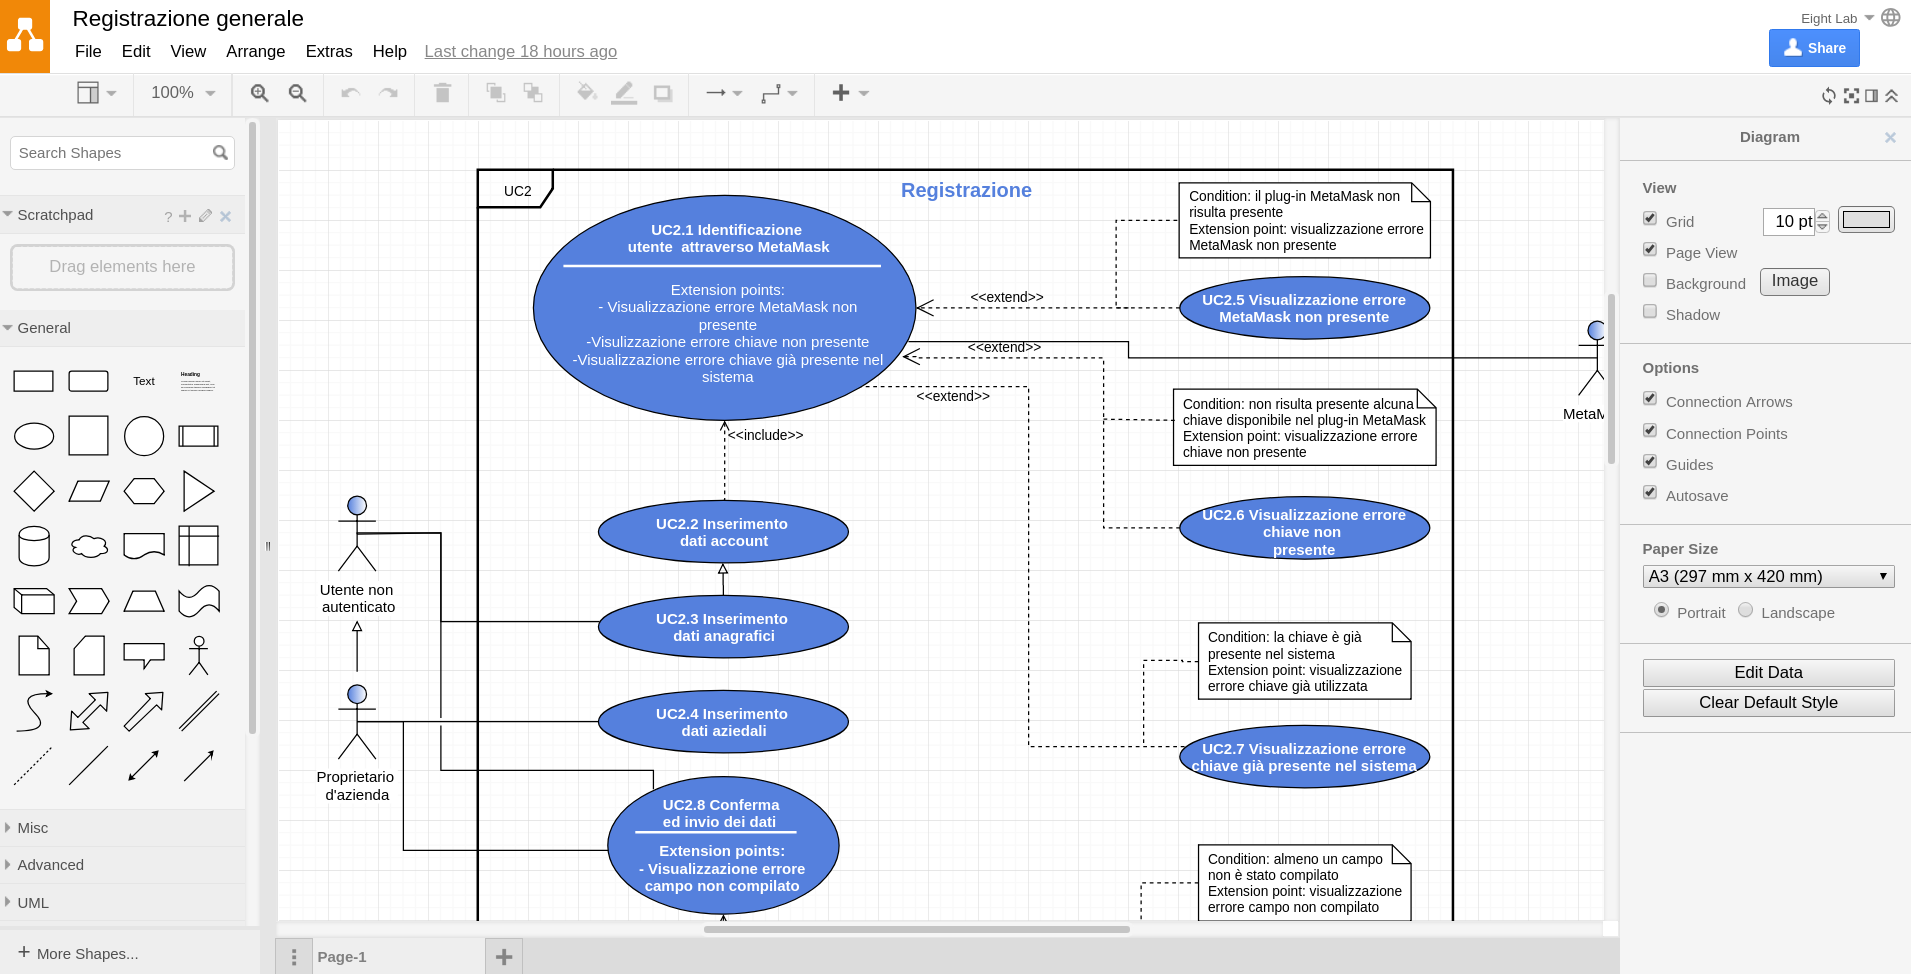
\includegraphics[width=0.99\linewidth]{res/images/drawio.png}
			\caption{Software per la creazione di diagrammi online}
		\end{figure} 
		\paragraph{IntelliJ IDEA} \mbox{}\\
		IntelliJ IDEA viene utilizzato per la codifica in Java e JavaScript. Questo IDE offre piena compatibilità con Linux, Windows, macOS, oltre ad essere un potente editor con molte funzionalità integrate.
		\url{https://www.jetbrains.com/idea/}
		\begin{figure}[H]
			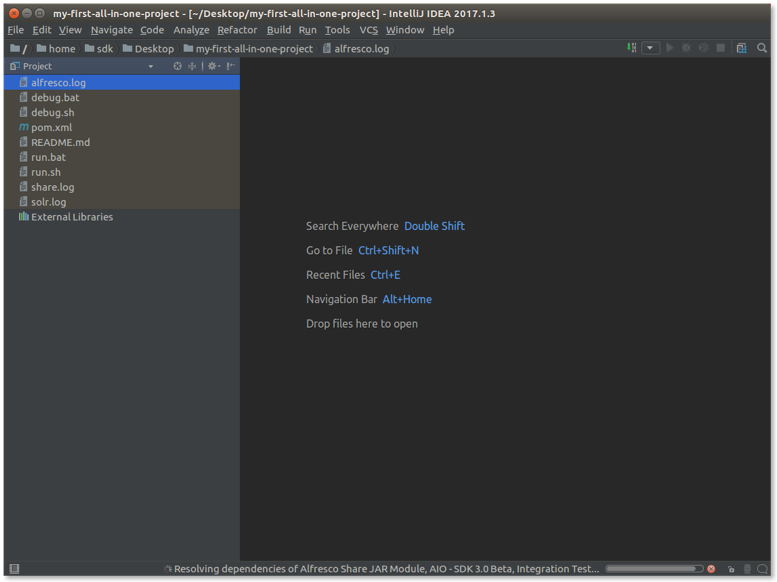
\includegraphics[width=0.99\linewidth]{res/images/intellij.png}
			\caption{Software per la codifica}
		\end{figure} 